
\cleardoublepage

\chapter{System Design}
\label{chapter:system_design}

The mapping system consists of the various components needed to capture, organize and locate images of the field, as well as any additional field items needed for identifying plants.  The proper design of the mapping system is the most important step in the overall mapping process.  Poor design leads to insufficient image quality, missing field coverage or improperly located images, which no amount of post-processing can correct.  

The first part of the system discussed is the markers used for plant identification because the required size of these markers impose constraints on the rest of the system.  Next, the base platform and additional equipment, such as cameras, is presented along with reasoning about nominal parameters such as vehicle speed and the camera height above the ground.  This chapter concludes by describing additional field markers which are not strictly necessary, but help improve the robustness of the mapping process. 

\section{Plant Identification}
\label{section:plantid}

As mentioned in the introduction chapter, the mapping process involves not just determining plant coordinates, but also assigning each plant to a group.  Each plant group is referenced by a unique identifier (ID), such as 1035.  The method used in this research is to encode this ID in a two-dimensional barcode that is placed at the beginning of each group of plants in the field. 

If a plant group needs to be planted in different parts of the field then a repetition letter is appended to the group number.  For example, three codes containing the text 1035A, 1035B and 1035C all belong to plant group 1035.  Since the two-dimensional barcodes are only placed at the beginning of the group it's critical to know the direction each row is planted in order to associate the correct set of plants with the plant ID.  Codes could be placed on both sides of each group to remove this added challenge, but this doubles the amount of code construction time, field debris and chance of missing a code during the post-processing.  Instead the row direction is encoded in row markers which is discussed later in this chapter.

\subsection{Code Format}
\label{section:code_format}

For this research project, Quick Response (QR) codes were selected as the barcode format. This is a standardized format that was made publicly available by Denso Corporation over 20 years ago.  It was first used for item tracking in the Japanese automotive industry, and has most recently become well known for encoding Uniform Resource Locators (URLs) for websites. <TODO ref article>.  Two important characteristics of this format is it can be read from any orientation, and it can still be read if part of the code is damaged.  Various other types of formats, such as Aztec or Micro QR, can encode information in smaller grids by restricting the character encoding, but offer less error correction.  Also, at the time this research was conducted these alternate formats were not supported by any of the open-source readers that the researcher investigated. 

\begin{figure}[htb]
	\centering
    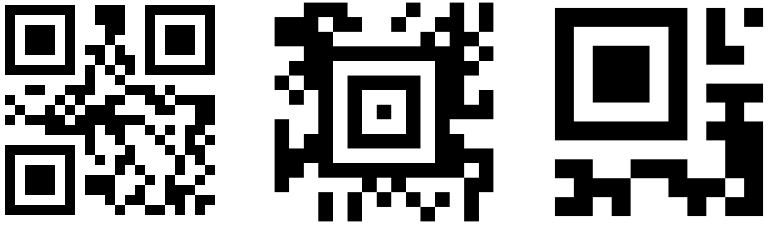
\includegraphics[width=3in]{figures/generated_codes_1035.png}
    \caption[2D barcode formats]{Comparison of 2D barcode formats encoding the text 1035 with high error correction.  From left to right: Quick Response (QR), Aztec and Micro QR.}
    \label{barcode_formats}
\end{figure} 

\subsection{Size Constraint}

For fields with thousands of different plant groups it's not feasible to place these QR codes by hand.  Therefore, they must fit through the deposit cylinders of the transplanter shown in figure <TODO ref experiment>.  In order to not get caught in the cylinders the codes cannot be larger than 2.5 centimeters in diameter. Since there needs to be a white margin around the actual QR code, the code itself ends up being roughly 2 centimeters.  The QR code format is split into different versions which define how many squares make up the code.  The first version is a grid of 21 by 21 squares and is shown in figure \ref{barcode_formats}.  This results in a maximum square size of only 1 millimeter.  

\subsection{Code Construction}

The codes must be easy to produce due to the potentially large number of codes required for each field.  The <TODO> program can be used to generate all QR codes at once, and a thermal printer can print the codes on pot labels rapidly.  However, the pot labels need a solid base to stay upright and grounded during transplanting. The researchers at the Land Institute in Salina, Kansas, developed a biodegradable base <TODO better describe base> that the pot labels are inserted into.  An example of one of these QR codes can be seen in figure \ref{QR_code}.

\begin{figure}[htb]
	\centering
    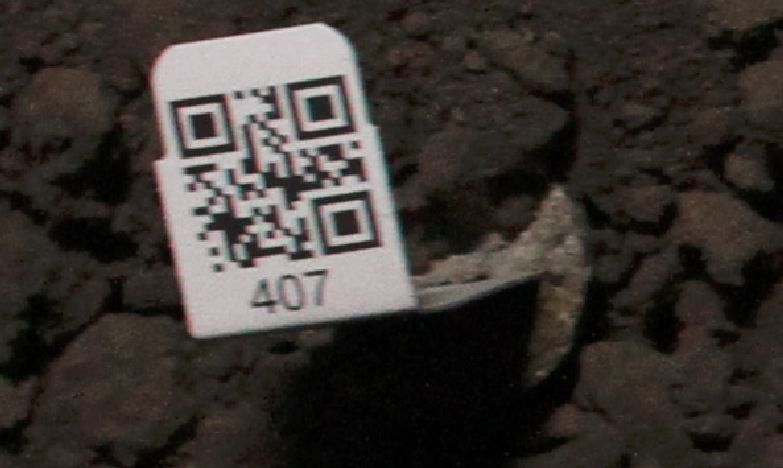
\includegraphics[height=2in]{figures/qr_code_407.png}
    \caption[QR code]{QR code printed on pot label and planted in field.}
    \label{QR_code}
\end{figure}

\section{Platform Design}
\label{section:platform_design}

There are many types of platforms that could be used for mapping.  Aerial vehicles have the benefit of autonomously traversing the field without the possibility of running over plants. However, they are unable to provide external lighting or shading which is important when post-processing the images. In addition, the size constraint on QR codes would require low altitude flights at a constant altitude to keep the codes properly focused, which is not easy to achieve.  Higher altitude flights would be possible with a telescopic lens, but this increases cost, weight and most critically the effects of error in camera orientation.  For these reasons only ground platforms are considered.

Two different types of ground platforms are investigated, a manual push-cart and a four-wheel robotic vehicle.  The push-cart excels in it's simplicity, however for this thesis only the robotic platform is discussed.  The main benefits of a robot is the ability to drive at a constant speed and the option to operate autonomously.  Driving at a constant speed is important to ensure sufficient overlap between successive images, and self-driving vehicles remove much of the tedious work associated with imaging large fields.  

\subsection{Robotic Platform}

The selected robotic platform is the Husky A2000 mobile robot made by Clearpath Robotics.  The Husky is a four wheeled differential drive robot measuring 39 inches in length and 27 inches wide.  It features a maximum speed of 1 meters per second and can carry up to 75 kilograms.  A custom C-channel structure was added to the top of the robot to enable it to image the field.  This structure can be seen in figure \ref{husky_rocky_ford}.  Attached to the front of the structure are two Canon 7D digital single-lens reflex (DSLR) cameras.  Using two cameras allows two rows to be mapped at the same time. 

\begin{figure}[htb]
	\centering
    \includegraphics[height=2.7in]{figures/sunflower_rocky_ford_labeled.jpg}
    \caption[Husky]{Husky A2000 mobile robot equipped with two cameras.}
    \label{husky_rocky_ford}
\end{figure}

On the back of the C-structure are two white Trimble AG25 antennas, which attach to a Trimble BX982 global navigation satellite system (GNSS) receiver.  This receiver is mounted to the top of the robot.   

\subsection{GNSS Receiver}

The BX982 receiver provides centimeter level accuracy when paired with a fixed base receiver broadcasting RTK correction signals.  For this application the fixed base is a Trimble Ag542 receiver with a Trimble Zypher Geodetic antenna as shown in figure \ref{base_station}.  This base station communicates with the SNB900 rover radio mounted on the robot over a 900 MHz radio link.   The dual antenna design allows the robot to determine its heading, or yaw, to within approximately 0.1 degree.  This accurate yaw is important for geo-locating plants and QR codes within images, as well as allowing the robot to operate autonomously as discussed in section \ref{section:automated_control}. 

\begin{figure}[htb]
	\centering
    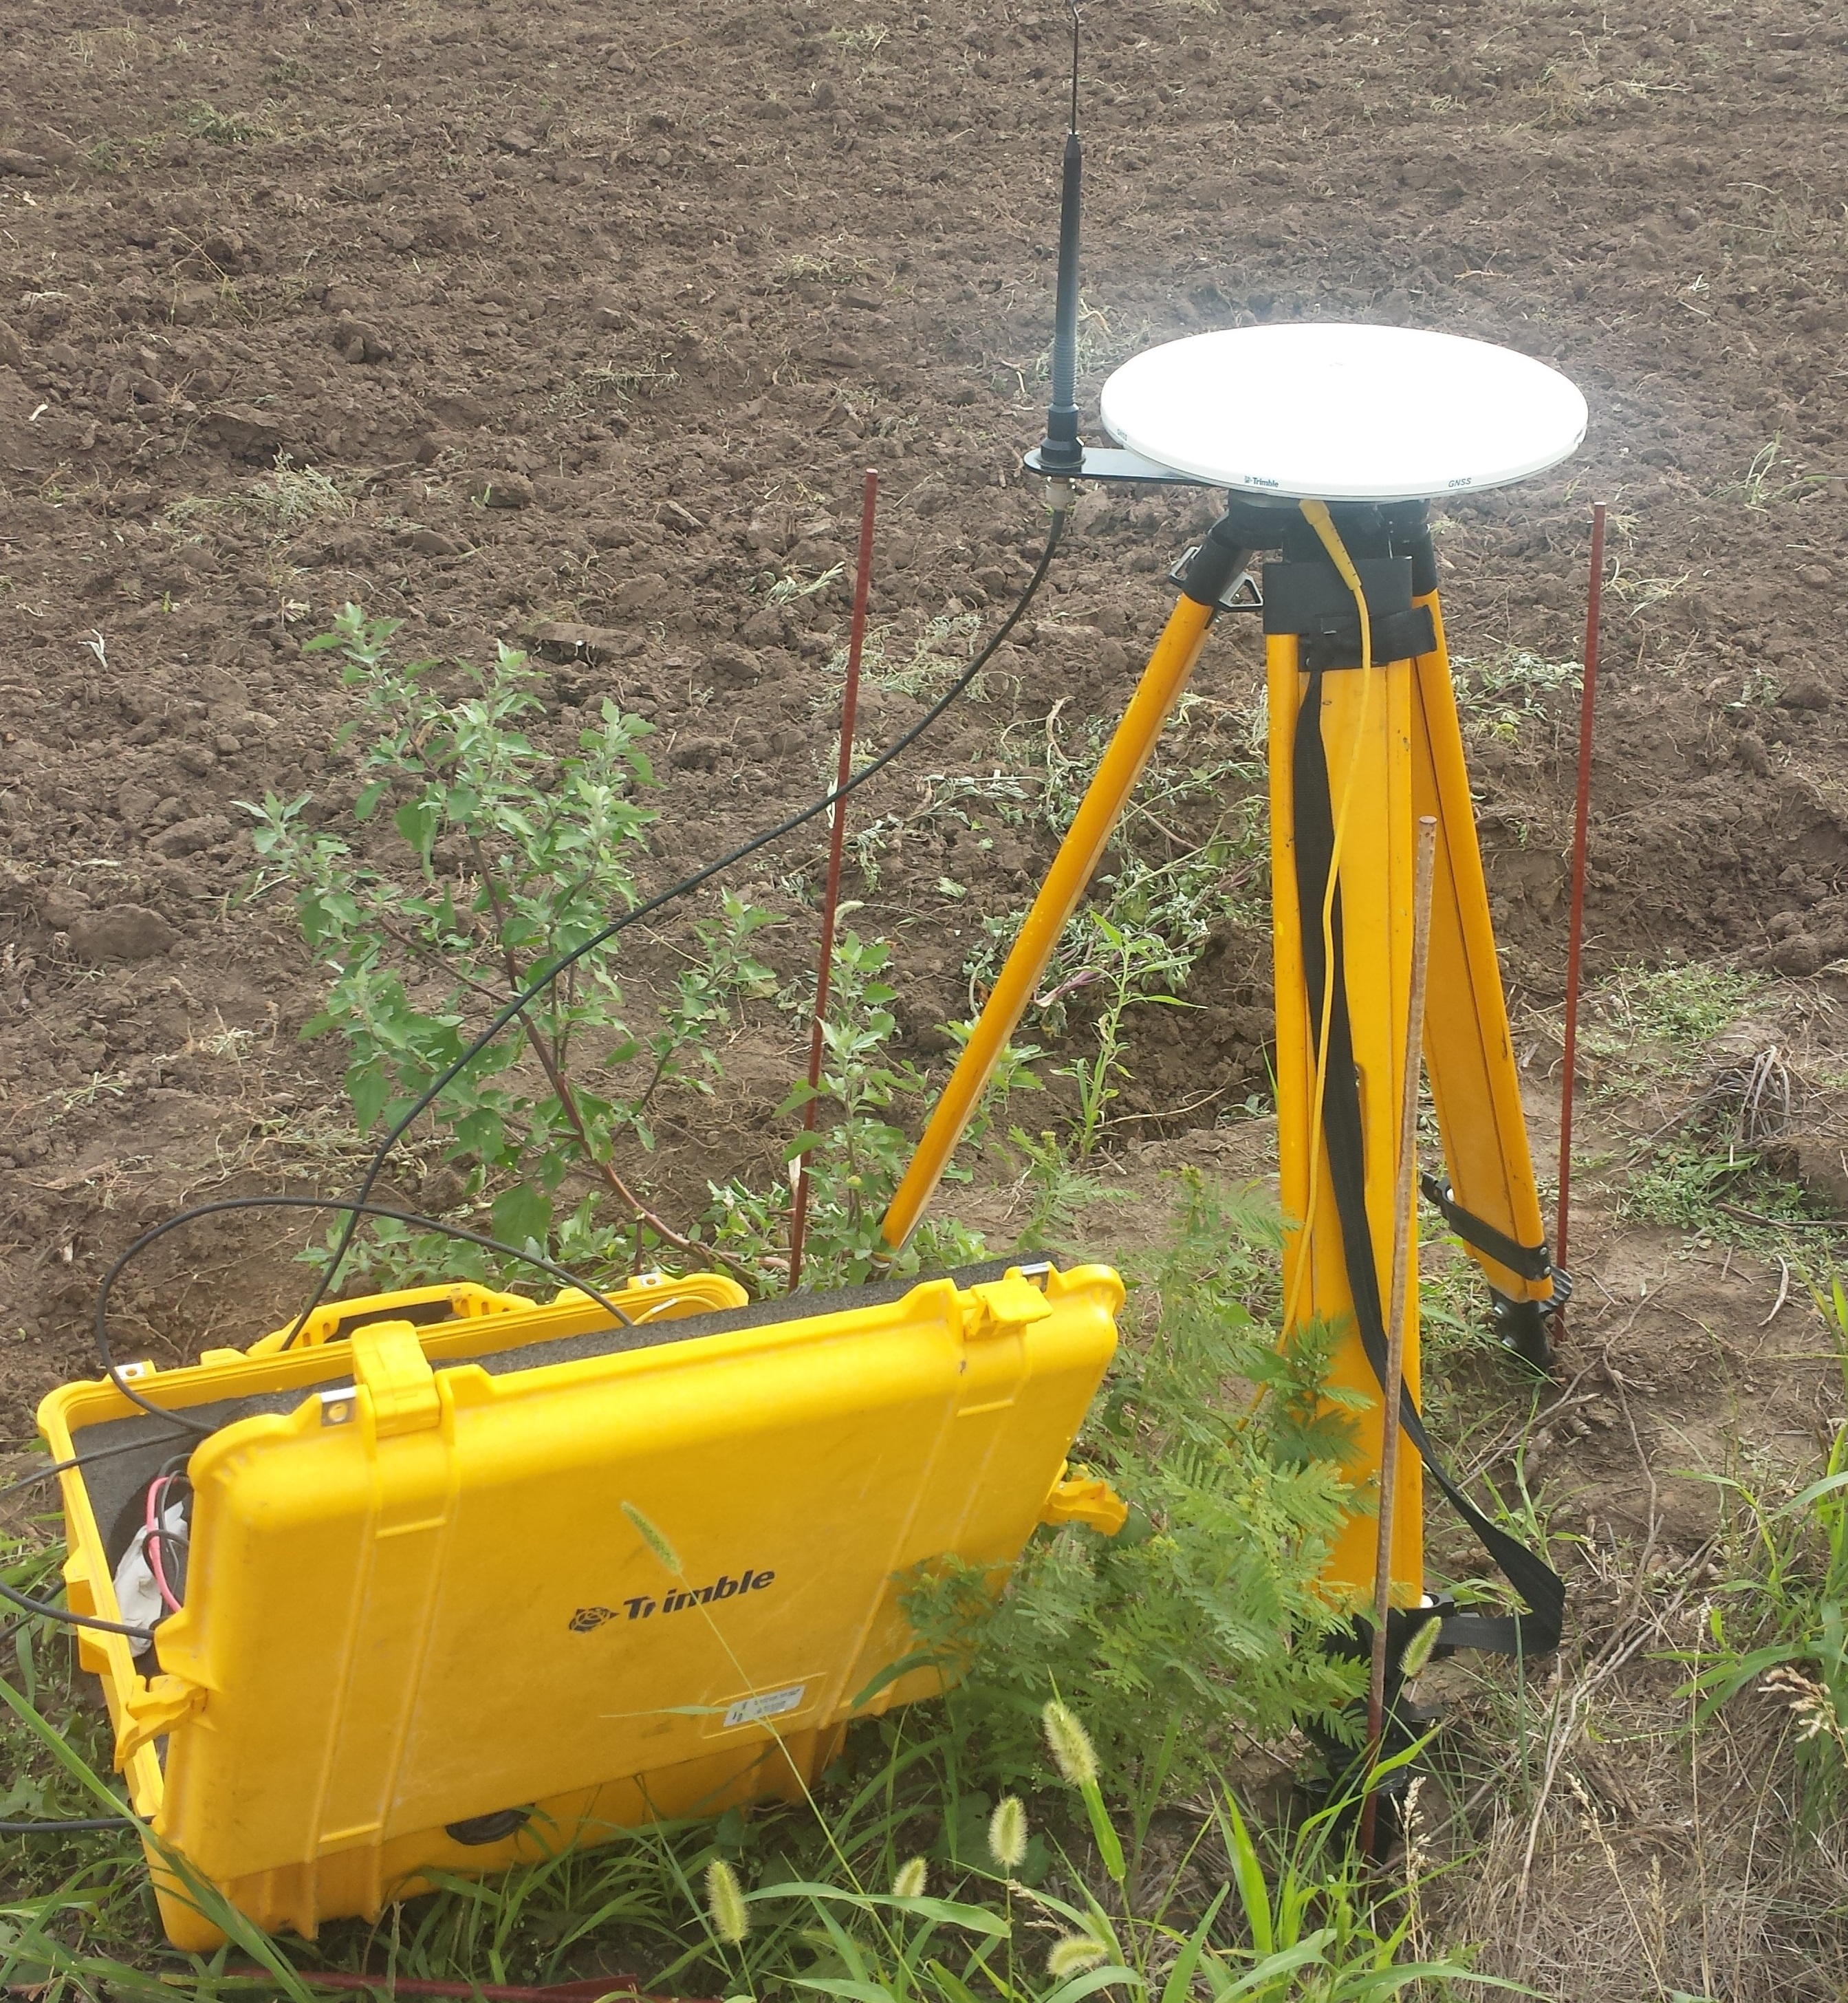
\includegraphics[height=3in]{figures/sunflower_base_cropped.jpg}
    \caption[Base station]{Ag542 base station mounted on tripod.}
    \label{base_station}
\end{figure}

\subsection{Cameras and Lighting}

The Canon 7D features an 18 megapixel (MP) sensor and is fitted with a fixed 20 millimeter focal length wide-angle lens.  The camera contains an Advanced Photo System type-C (APS-C) sensor rather than a full frame 35mm sensor. When paired with the wide-angle lens this gives a horizontal angle of view of 58.3 degrees and a vertical view of 40.9 degrees.  
As shown in figure \ref{husky_rocky_ford} the cameras are mounted far out in front of the robot so that the wheels and front bumper do not show up in the image and effectively reduce the field of view.  In addition, each camera is mounted with a 90 degrees yaw offset with respect to the platform so that the longer side of the image is aligned with the forward movement of the robot as seen in figure \ref{figure:image_fov}.  

\begin{figure}[htb]
	\centering
    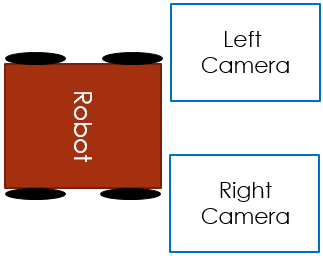
\includegraphics[height=2in]{figures/camera_directions.png}
    \caption[Camera field of view]{Depiction of camera field of views relative to robotic platform.}
    \label{figure:image_fov}
\end{figure}

An item that is not pictured on the robot, but is shown in figure \ref{figure:canon_and_bars} is a light emitting diode (LED) bar.  These 9 watt bars provide external lighting at night time for consistent image lumination.  It is feasible to only use 2 bars, one for each camera, however using 4 bars provides enough light for the camera settings to be set conservatively.  Another benefit of using one bar on each side of each camera is it noticeably reduces image glare on the QR codes.  

\begin{figure}[htb]
	\centering
    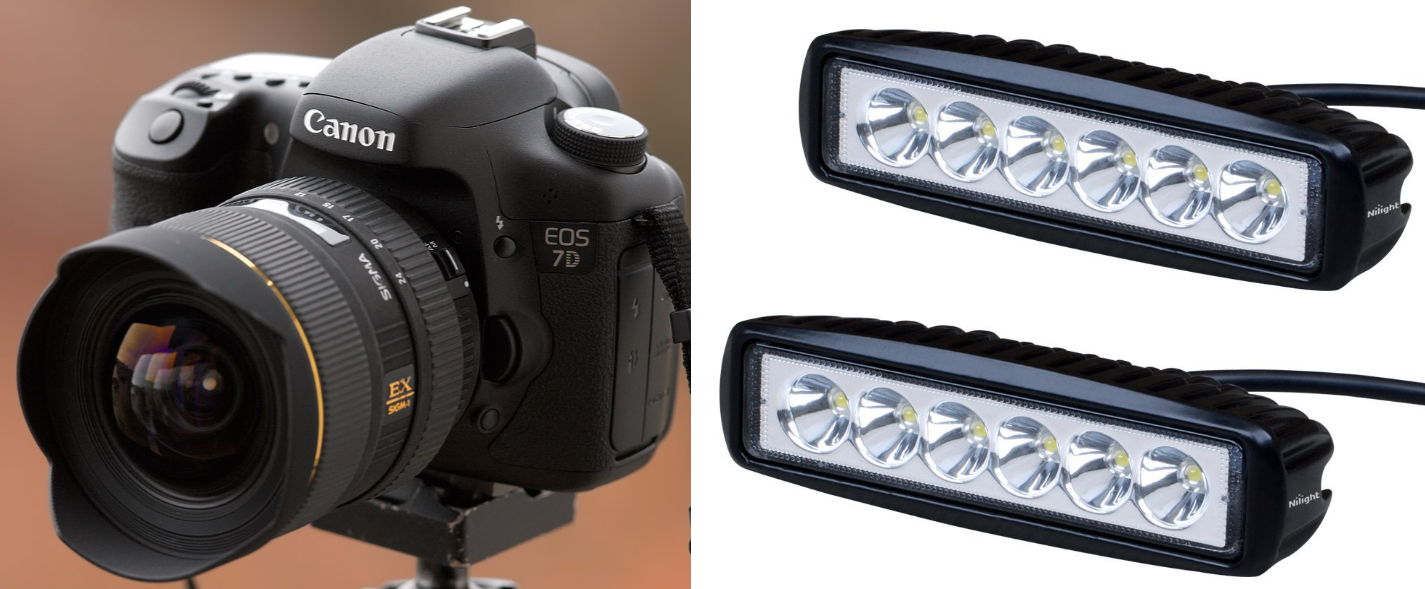
\includegraphics[height=2in]{figures/canon7d_and_LEDs.png}
    \caption[Canon 7D and LED bars]{Canon 7D and external lighting bars.}
    \label{figure:canon_and_bars}
\end{figure}

\subsection{Determining Parameters}

There are many parameters, such as camera height and vehicle speed, which are chosen to ensure quality images and sufficient field coverage.  The most important to determine first is the camera height, as that determines the resolution of the image.  If the image resolution is too low then the QR codes will be unreadable.  
If each pixel could correspond to exactly one square on the QR code then the minimum resolution would be 1 pixel per millimeter, since each square is roughly 1 millimeter in size.  In reality this is almost never the case, and the theoretical minimum is 3 pixels for one square.  If only 2 pixels per square are used then the light from the square could be split in half with the adjacent white square and the result would be an unresolved gray square.  However, all lenses also introduce some loss in contrast.  The amount of contrast lost is a function of many things such as lens diffraction, aperture and pixel position.  Also in reality the camera's optical axis is not always perfectly orthogonal to the QR code.  To account for these extra effects the actual minimum resolution is set to 5 pixels per millimeter.  

The 18 million effective pixels on the sensor are split into a 5184 by 3456 grid.  The minimum resolution then requires a maximum image size of 1037 by 690 millimeters, which constrains the cameras to be no higher than 930 millimeters above the QR codes.  In order to make the imaging process more robust, the cameras are mounted 700 millimeters above the ground which corresponds to an image size of 781 by 520 millimeters, and a resolution of approximately 6.5 pixels per millimeter.  Mounting the cameras lower than the maximum requirement also always the external lighting to be more concentrated and requires smaller shading if the imaging is done during the day.  

Another requirement that is added to make the mapping process more robust is each QR code must be in a minimum of two images.  This helps solve temporary issues such as bugs flying in front of the camera as well as offers multiple perspectives if the code is accidentally planted at an angle.  In order to ensure this the maximum spacing between successive images is given by the equation
\begin{align*}
 \text{max spacing} &= (\text{image width} - \text{QR side length} - \text{pad}) / 2 \\
             &= (781 - 25 - 75) / 2 \\ 
             &= 340 \text{ millimeters}
\end{align*}
where the pad is extra spacing to account for variations in camera latency and reduced lighting at the image border.
  
An additional constraint on the cameras that must be taken into account is the minimum trigger period.  Many cameras, including the Canon 7D, are capable of exposing images rapidly and then buffering them before they are processed.  However, the minimum trigger period considered in this section is the minimum amount of time for an image to be exposed, processed and saved without continued buffering, as buffering can only be sustained for so long.  This was experimentally determined for the Canon 7D to be 0.7 seconds.  

In order to satisfy the maximum image spacing, while not exceeding the minimum trigger period, the robot cannot drive faster than 0.5 meters per second.  One downside of driving this fast is cameras begin to noticeably shake when the field is not smooth, which can lead to blurry images.  Therefore the nominal robot speed is set to 0.4 meters per second.  These platform parameters are summarized in table \ref{table:platform_params}.

\begin{table}[htb]
    \begin{center}
    \caption{Summary of platform parameters.}
    \begin{tabular}[c]{|c|c|c|}
        \hline
        Parameter & Value & Units \\
        \hline
        Camera Height    & 700       & millimeters         \\
        Image Size       & 781 x 520 & millimeters         \\
        Image Resolution & 6.5       & pixels / millimeter \\
        Trigger Period   & 0.7       & seconds / image     \\
        Robot Speed      & 0.4       & meters / second     \\
        \hline
    \end{tabular}
    \label{table:platform_params}
   \end{center}
\end{table}

\subsection{On-board Computers}

There are a total of four computers used on the Husky.

\begin{description}
\item[Main Husky Computer] - custom mini-ITX situated inside the main compartment of the robot running Ubuntu 12.04 along with the Robot Operating System (ROS). This computer contains all of the telemetry and guidance logic and is discussed more in section \ref{section:base_functionality}.  
\item[Husky Microcontroller] - Atmel ARM-based SAM7XC256 enclosed in the back of the robot chassis.  This microcontroller receives linear and angular velocity commands from the main computer and reports feedback from the robot's encoders, battery and motors. 
\item[Husky Interface Computer] - Lenovo T400 laptop that is also running Ubuntu 12.04 along with ROS.  This computer sits on top of the Husky and is used to send commands to the robot using a secure shell (SSH)
\item[Data Collection Computer] - Lenevo S431 laptop running Windows 7 that also sits on top of the Husky.  This computer runs the program responsible for saving data from the cameras and GNSS receiver.   
\end{description}

For simplicity the output of the GNSS receiver is split to both the data collection computer as well as the main Husky computer.  It would be ideal to run the data collection program on the Husky interface computer to eliminate the need for an extra computer.  However, the data collection program requires a Windows based operating system to interact with the Canon cameras, and at the time of this research ROS is not stable on Windows. 

\section{Guidance and Control}

The Husky arrived from Clearpath with basic driving functionality, however this was not sufficient for the mapping process.  This section describes the additional functionality developed for the robot that enables it to operate in autonomous or semi-autonomous modes.  

\subsection{Base Functionality}
\label{section:base_functionality}

When the Husky was purchased the main computer came installed with the Robot Operating System, which is popular open-source framework that provides many of the same services as traditional operating system such as inter-process communication and hardware-abstraction.  One major benefit is ROS allows different functionality to be split up into separate processes, referred to as nodes.  This promotes code re-use and prevents one component from crashing the entire system.   The nodes that were pre-installed on the Husky are listed below.

\begin{description}
\item[Teleop node] - receives driving commands from the Logitech controller shown in \ref{figure:cruise_control}.  The default functionality is when the X button is held down and the left and right analog sticks command linear and angular velocity, respectively.
\item[Husky node] - in charge of sending the velocity commands over a serial port to the microcontroller that controls the motors.  
\item[IMU node] - driver for the UM6 orientation sensor that came installed on the robot.  However, this node is not used since the platform is stable and the multiple GNSS antennas determine yaw.
\end{description}

\subsection{Cruise Control}

When driving through the field it's important that the robot maintains a constant speed to ensure all QR codes and plants are imaged.  With the basic teleop functionality this was difficult to achieve while also keeping the robot centered in the middle of the row. To solve this issue the researcher extended the teleop node to include cruise control functionality that is commonly seen in automobiles.  

\begin{figure}[htb]
	\centering
    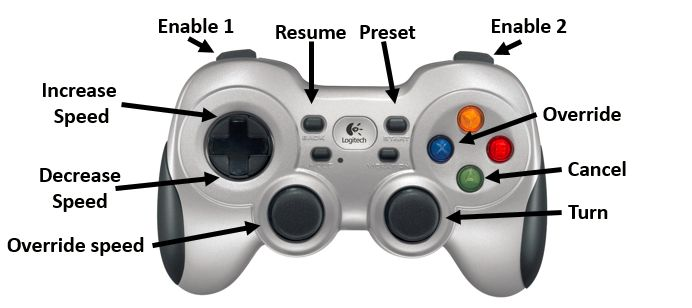
\includegraphics[height=3in]{figures/logitech_controller_labelled.png}
    \caption[Cruise control buttons]{Logitech controller for Husky showing cruise control functionality.}
    \label{figure:cruise_control}
\end{figure}

Cruise control can be enabled by either pressing both the Enable 1 and Enable 2 buttons at the same time or by the Preset button.  The Preset button defaults to a certain configuration speed, by default 0.4 meters per second.  If the Override button is pressed then the linear speed is temporarily determined from the left analog stick, as is the case in basic driving mode.  The Resume button returns to the last speed, if there was one, and the up and down arrows on the D-pad vary the commanded speed in increments of 0.05 meters per second.    

\subsection{Automated Control}
\label{section:automated_control}

While this cruise control feature makes it feasible to manually drive the robot through the field, for large experiments this is a tedious task that requires ten or more hours of keep the robot centered between the rows.

ROS contains well-developed navigation functionality that allows the robot to convert odometry and sensor data into velocity commands for the robot.  This navigation code, however, is based around advanced functionality such as cost maps, detailed path planning and map-based localization. All of which are unnecessary for this application.  Therefore, the researcher decided to develop a simple guidance solution that is implemented in the following nodes

\begin{description}
\item[GPS node] - combines position and yaw data from the GNSS receiver and publishes this data to the rest of the ROS system.
\item[Waypoint upload node] - allows the Husky interface computer to load a set of waypoints into to robot.
\item[Guidance node] - computes robot velocity needed to follow a set of waypoints. 
\end{description}

\section{Data Collection Software}
\label{system-software}

A critical part of the mapping process is being able to accurately associate each image with the position and orientation of the camera at the time the image was taken.  This process was accomplished using the Dynamic Sensing Program (DySense), which is an open-source data collection program that provides the means to obtain, organize and geo-locate sensor data.  This program was developed by the researcher in order to standardize data collection across various types of platforms and sensors.  A screen shot of DySense can be seen in figure \ref{dysense_screenshot}.

Similar to how ROS splits different functionality into processes, DySense can split sensor drivers into processes, which allows them to be written in any programming language.  The camera sensor driver is written in C\# and uses the EOS Digital Software Development Kit (EDSDK) to interact with the camera.  This driver allows the images to be downloaded from the camera in real-time and assigns each one a unique file name and an estimated UTC time stamp of when the image was exposed.

\begin{figure}[htb]
	\centering
    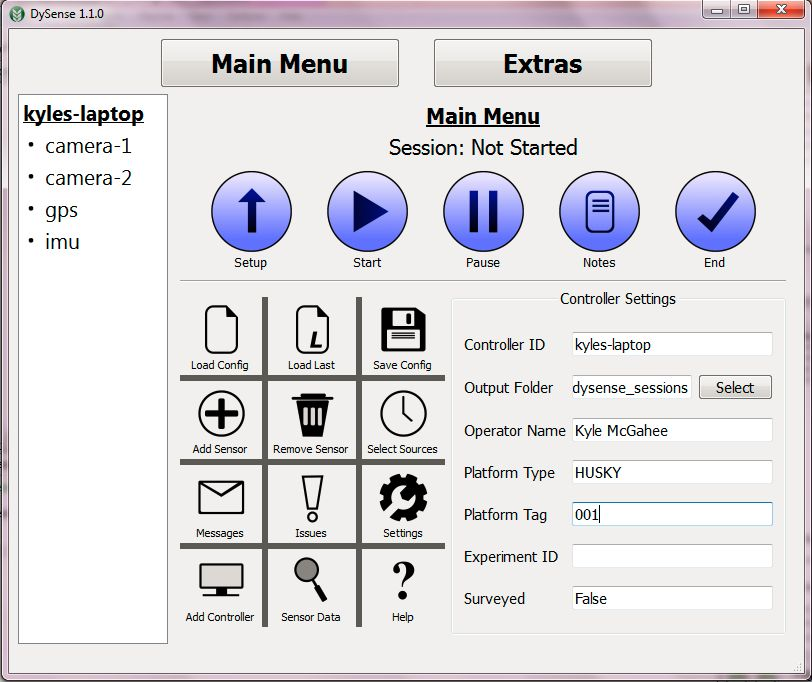
\includegraphics[height=4.5in]{figures/dysense2.png}
    \caption[Data collection program]{Screenshot of the data collection program.}
    \label{dysense_screenshot}
\end{figure}

DySense also uses GPS and IMU drivers to record the platform's position and orientation.  This knowledge of the platform state, as well as the camera offsets in the platform frame, allows the positions and orientations of each camera to be calculated at the same time as every image.    

\section{Additional Markers}
\label{system-markers}

In addition to the group QR codes there are two other types of markers used in the mapping process, row markers and plant markers.   

\subsection{Row Markers}

Row markers are placed at the beginning and end of each row. Similar to identifying plant groups, these markers are also implemented using QR codes.  These row codes store the row number and signify whether the code is the start ("St") or end ("En") of the row. As discussed in section \ref{section:plantid}, it is critical to know the planting direction of each row because that defines which plants are associated with each group QR code.

\begin{figure}[htb]
	\centering
    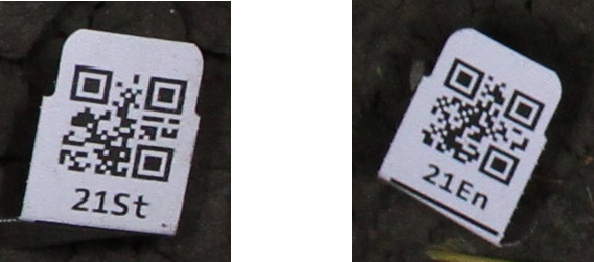
\includegraphics[height=2in]{figures/row_codes.png}
    \caption[Row QR codes]{QR codes marking the start and end of row 21.}
    \label{figure:row_codes}
\end{figure}

\subsection{Plant Markers}
\label{section:plant_markers}

The second type of marker is used to help distinguish regular plants from other plant debris that may be found in the field after tilling <TODO is this the right word?>.  This marker is optional, but helps improve the robustness of locating plants.  Depending on the size and quality the field these markers can be used on every plant or, for example, every 4 plants. 

The marker used in this experiment is a blue dyed wooden stick approximately 5 inches in length, which is placed in the center of each plant. The color blue is selected because it provides the largest difference between other hues likely found in the field, such as yellow/green in plants and red in soil.  In addition to marking the plants, this stick also helps prevent the plants from flipping over when exiting the planter.

Another type of plant marker worth mentioning is a colored tag pierced through the top of an un-dyed wooden stick.  This type of marker can provide addition information for manual plant inspection and is much more saturated than the dyed sticks, making it easier to detect. 

\begin{figure}[htb]
	\centering
    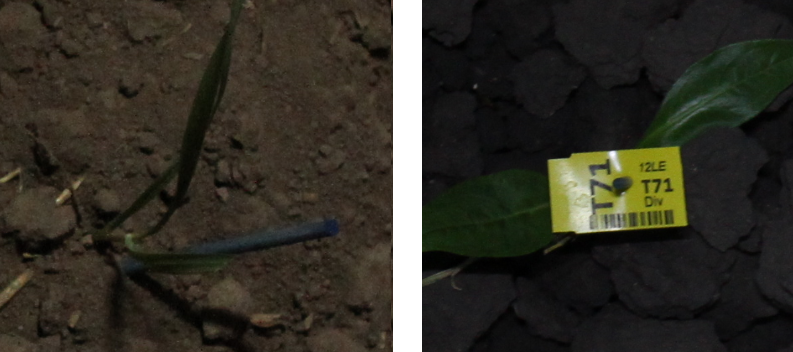
\includegraphics[height=2.5in]{figures/plant_markers.png}
    \caption[Plant markers]{Examples of blue stick (left) and colored tag (right)}
    \label{figure:plant_markers}
\end{figure}
